\chapter{Les ondes}\label{Ch-ondes}
\begin{abstract}
Jusqu'ici, nous n'avons quasiment pas parlé de mode propre cela est plus ou moins évoqué à travers, par exemple, «la plus petite période du système» au chapitre précédent... mais cela a été fait à dessein.

En effet, nous avons voulu, dans ce chapitre, regrouper les approches modales, car cela nous a semblé plus en cohérence.
\end{abstract}

\medskip
\section{Introduction}
Dans la mesure où se document s'adresse à des ingénieurs en mécanique (ou en acoustique), la notion de mode propre est une notion relativement maîtrisée.

\bigskip
Un système mécanique atteint un \textcolorblue{mode propre de vibration}\index{mode propre} lorsque tous les points de ce système sont à une fréquence donnée appelée \textcolorblue{fréquence propre}\index{fréquence propre} du système. Une fréquence propre est \textcolorblue{fondamentale} si elle n'est pas le multiple d'une autre fréquence propre; dans le cas contraire, c'est une \textcolorblue{harmonique}.

\medskip
On appelle \textcolorblue{résonance}\index{résonance} le phénomène selon lequel certains systèmes physiques sont particulièrement sensibles à certaines fréquences. Un système résonant peut accumuler une énergie, si celle-ci est appliquée sous forme périodique, et proche d'une fréquence propre. Soumis à une telle excitation, le système est alors le siège d'oscillations de plus en plus importantes, jusqu'à atteindre un régime d'équilibre qui dépend des éléments dissipatifs du système, ou bien jusqu'à rupture d'un composant du système.

\medskip
Si l'on soumet un système résonant à une percussion (pour les systèmes mécaniques) ou à une impulsion (pour les systèmes électriques), et non plus à une excitation périodique, alors le système sera le siège d'oscillations amorties sur des fréquences proches de ses fréquences propres et retournera progressivement à son état stable. \textcolorgreen{Physiquement, c'est le coup de marteau de choc donné sur une structure pour en déterminer les modes.}

\medskip
Un système susceptible d'entrer en résonance, i.e. susceptible d'être le siège d'oscillations amorties, est un \textcolorblue{oscillateur}\index{oscillateur}. Un tel système a la particularité de pouvoir emmagasiner temporairement de l'énergie sous deux formes: potentielle ou cinétique. L'oscillation est le phénomène par lequel l'énergie du système passe d'une forme à l'autre, de façon périodique.

Si l'on injecte une énergie potentielle au moment où l'énergie potentielle déjà emmagasinée est maximale, l'énergie ainsi injectée s'ajoute à l'énergie déjà emmagasinée et l'amplitude de l'oscillation va augmenter, ainsi que l'énergie totale. Idem pour l'énergie cinétique. Ainsi, si l'on apporte de l'énergie avec une périodicité égale (ou proche) de la périodicité propre du système, l'énergie totale va augmenter régulièrement et l'amplitude des oscillations du système va ainsi croître. L'exemple le plus simple est celui d'une balançoire: l'énergie de chaque poussée s'ajoute à l'énergie totale, à condition de pousser au bon moment...

Le phénomène de \textcolorblue{résonance}\index{résonance} n'est rien d'autre que cet effet d'accumulation de l'énergie en injectant celle-ci au moment où elle peut s'ajouter à l'énergie déjà accumulée, i.e. «en phase» avec cette dernière.

\medskip
Quand l'excitation aura cessé, le système résonant sera le siège d'\textcolorblue{oscillations amorties}: il va revenir plus ou moins vite à son état d'équilibre stable. En effet, l'énergie de départ sera peu à peu absorbée par les éléments dissipatifs du système (amortisseur visqueux en mécanique, résistances en électricité...). Un système peu amorti sera le siège d'un grand nombre d'oscillations qui diminueront lentement avant de disparaître complètement.

\medskip
La \textcolorblue{représentation modale}\index{représentation modale} est pertinente dans le domaine des basses fréquences, i.e. pour les premiers modes propres.\index{mode propre} Dans les domaines moyennes et hautes\\
 fréquences, on utilise des méthodes adaptées à la \textcolorblue{densité spectrale}\index{densité spectrale} élevée.

Les domaines moyennes fréquences et hautes fréquences sont définis par la densité spectrale.\index{densité spectrale} En effet, l'expression en fréquences n'a pas de sens pour définir ces domaines, une similitude sur un système physique modifie les fréquences propres\index{fréquence propre} mais le spectre reste semblable, à un facteur près. Dans le cas de fréquences multiples, il existe un sous-espace propre donc les modes propres\index{mode propre} sont arbitraires dans ce sous espace. Dans le cas de fréquences voisines (densité spectrale élevée),\index{densité spectrale} la représentation modale\index{représentation modale} n'est pas robuste car de faibles perturbations du domaine physique vont entraîner un changement important des modes propres\index{mode propre} associés à ces fréquences. \textcolorblue{Donc la représentation modale n'est pertinente que pour le domaine des basses fréquences, domaine défini par la densité spectrale.} Le domaine basses fréquences s'étendra jusqu'à quelques Hz en génie civil, jusqu'à des milliers de Hz pour de petites structures mécaniques.

\medskip
Le phénomène de \textcolorblue{synchronisation},\index{synchronisation} ou \textcolorblue{accrochage de fréquences} est un phénomène par lequel deux systèmes excités chacun selon une fréquence se mettent à osciller selon la même fréquence. On trouve de nombreux exemples de ce phénomène dans la nature:
\begin{itemize}
  \item Le plus connu et le plus facilement observable concerne la Lune: celle-ci présente toujours la même face à la Terre. Cela signifie que la période de rotation de la Lune sur elle-même~$T_0$ est égale à la période de rotation de la lune autour de la Terre~$T\cong 28$~jours. Il s'agit d'une résonance 1:1. L'analyse montre que ce n'est pas une coïncidence, et que cela est dû à un faible couplage gravitationnel entre ces deux mouvements.

  \item Le règne animal n'est pas en reste et fournit lui-aussi des exemples de synchronisation, auxquels on ne pense pas spontanément. Citons le vol d'oiseaux ou le clignotement des lucioles...
\end{itemize}

\medskip
\begin{histoire}
On trouve d'autre exemples historiques relatifs à ce phénomène de synchronisation. En voici deux parmi les plus connus.

\sbox{\MaBoiteAvecPhotos}{\setlength{\tabcolsep}{0pt}\scriptsize%
\begin{tabular}{c}
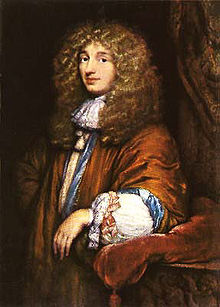
\includegraphics[height=\the\HauteurDesPhotos]{Huygens}\\
Huygens%
\end{tabular}}
\medskip
\ImageADroite{%
Le premier est celui de la synchronisation des balanciers de deux pendules accrochées au même mur d'une pièce. Un faible couplage par les vibrations transmises dans le mur, et une  dissipation faible, expliquent cet accrochage de fréquences et cette résonance 1:1.\\
\indent
	C'est Huygens\index[aut]{Huygens [ou Huyghens] (Christian), 1629-1695, Néerlandais} qui a remarqué et expliqué ce phénomène: le système composé des deux balanciers et du mur a deux fréquences voisines faiblement couplées, et il possède, par le couplage, deux modes propres correspondant aux mouvements en phase et en opposition de phase des deux pendules. C'est sur le premier mode\index{mode propre} que se produit la synchronisation.\index{synchronisation}
}

\sbox{\MaBoiteAvecPhotos}{\setlength{\tabcolsep}{0pt}\scriptsize%
\begin{tabular}{c}
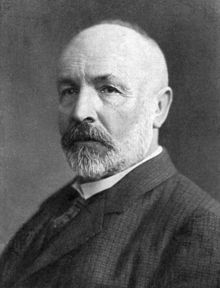
\includegraphics[height=\the\HauteurDesPhotos]{Cantor}\\
Cantor%
\end{tabular}}
%\medskip
\ImageAGauche{%
L'escalier de Cantor,\index[aut]{Cantor (Georg Ferdinand Ludwig Philip), 1845-1918, Allemand} ou escalier du diable est un exemple mathématique incontournable en analyse. Il correspond au graphe d'une fonction continue~$f$, sur~$\intff{0}{1}$, telle que~$f(0)=0$, $f(1)=1$, qui est dérivable presque partout, la dérivée étant presque partout nulle.\\
\indent
	L'escalier de Cantor peut également être vu comme la fonction de répartition d'une variable aléatoire réelle continue qui n'est pas à densité, et qui est même étrangère à la mesure de Lebesgue.\index[aut]{Lebesgue (Henri-Léon), 1875-1941, Français}\\
\indent
	Enfin, l'escalier du diable peut aussi être vu comme résultant d'un phénomène de 	synchronisation.\index{synchronisation} Si l'on change un paramètre extérieur du système de façon lente et continue, par exemple l'amplitude~$\alpha_0\in\RR$, alors la valeur de l'accrochage~$a=p/q$ va dépendre de ce paramètre. On obtient alors une fonction~$a(\alpha_0)$ de~$\RR \rightarrow \QQ$.
	Cette fonction très étrange comporte une multitude de paliers plus ou moins larges... et correspond à l'escalier du diable.
}
\end{histoire}
\medskipvm
En mathématiques, le concept de vecteur propre\index{vecteur propre|see{mode propre}}\index{mode propre} est une notion portant sur une application linéaire d'un espace dans lui-même. Il correspond à l'étude des axes privilégiés, selon lesquels l'application se comporte comme une dilatation, multipliant les vecteurs par une même constante.
Ce rapport de dilatation est appelé valeur propre;\index{valeur propre|see{fréquence propre}}\index{fréquence propre} les vecteurs auxquels il s'applique s'appellent vecteurs propres, réunis en un espace propre.\index{espace!propre}

\medskip
\begin{histoire}%
Bien qu'existant sous une forme non formalisée depuis longtemps, il aura fallu attendre l'invention des structures algébriques nécessaires pour vraiment pouvoir parler des valeurs propres\index{valeur propre|see{fréquence propre}}\index{fréquence propre} (issues par exemple de la cloture algébrique de~$\CC$ démontrée par Gauß).\index[aut]{Gauß (Johann Carl Friedrich), 1777-1855, Allemand}

\medskip
L'exemple immédiat qui vient à l'esprit est le traitement de l'équation de la chaleur\index{ED-EDP!de la chaleur} par Fourier\index[aut]{Fourier (Jean Baptiste Joseph), 1768-1830, Français} qui utilise déjà une base de vecteurs propres,\index{vecteur propre|see{mode propre}}\index{mode propre} bien que le concept n'ait pas encore été défini. Hamilton\index[aut]{Hamilton (William Rowan, Sir -), 1805-1865, Irlandais} introduira la notion de polynôme caractéristique, ce qui permet de déterminer ce que l'on appelle maintenant les valeurs propres\index{valeur propre|see{fréquence propre}}\index{fréquence propre} associées à l'endomorphisme d'une équation différentielle linéaire.

\sbox{\MaBoiteAvecPhotos}{\setlength{\tabcolsep}{0pt}\scriptsize%
\begin{tabular}{cccc}
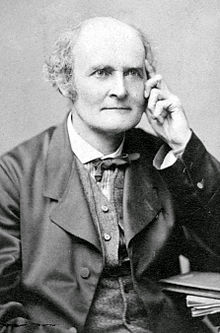
\includegraphics[height=\the\HauteurDesPhotos]{Cayley}&
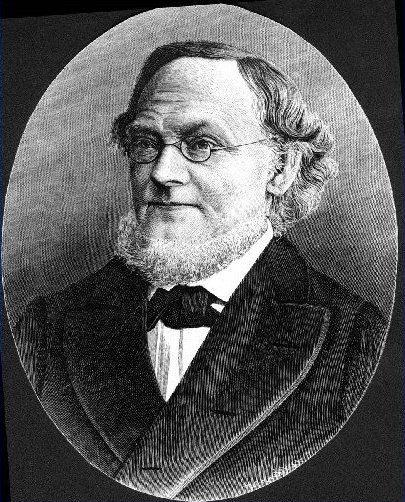
\includegraphics[height=\the\HauteurDesPhotos]{Grassmann}&
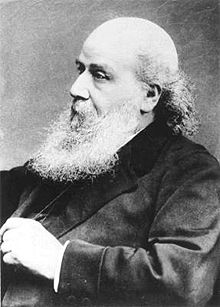
\includegraphics[height=\the\HauteurDesPhotos]{Sylvester}&
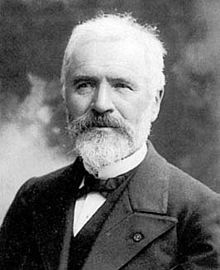
\includegraphics[height=\the\HauteurDesPhotos]{Jordan}\\
Cayley&Grassmann&Sylvester&Jordan%
\end{tabular}}
\medskip
\ImageADroite{%
Plusieurs aller-retour permettront de définir les notions d'espace vectoriel (Cayley,\index[aut]{Cayley (Arthur), 1821-1895, Anglais} Grassmann,\index[aut]{Grassmann (Hermann Günther), 1809-1877, Allemand} Cauchy),\index[aut]{Cauchy (Augustin Louis, baron -), 1789-1857, Français} de matrice (Sylvester,\index[aut]{Sylvester (James Joseph), 1814-1897, Anglais} Cayley)\index[aut]{Cayley (Arthur), 1821-1895, Anglais} et de valeurs propres\index{valeur propre|see{fréquence propre}}\index{fréquence propre} (Sylvester,\index[aut]{Sylvester (James Joseph), 1814-1897, Anglais} Jordan).\index[aut]{Jordan (Marie Ennemond Camille), 1838-1922, Français} Hilbert\index[aut]{Hilbert (David), 1862-1943, Allemand} finalement fera prendre conscience de la profondeur de la notion de valeur propre.\index{valeur propre|see{fréquence propre}}\index{fréquence propre} L'analyse fonctionnelle naît dans la foulée, et elle est l'objet de la première partie de ce document.}
\end{histoire}
\colorblack

\medskip
\section{Notions de valeur, vecteur, mode et fréquence propres}\index{valeur propre|see{fréquence propre}}\index{fréquence propre}\index{vecteur propre|see{mode propre}}\index{mode propre}\index{mode propre}\index{fréquence propre}

\medskip
Étant donné une matrice carrée~$\MM{A}$ d'ordre~$n$ \textcolorgris{(à coefficients dans un anneau commutatif)}, on cherche un polynôme dont les racines sont précisément les valeurs propres de~$\MM{A}$. Ce polynôme est appelé \textcolorblue{polynôme caractéristique}\index{polynôme! caractéristique} de~$\MM{A}$ et est défini par:
\begin{equation} p_A(X):=\det(X\MM{I}_n-\MM{A})\end{equation}
avec~$X$ l'indéterminée du polynôme et~$\MM{I}_n$ la matrice identité d'ordre~$n$.
\medskipvm
Si~$\lambda$ est une \textcolorblue{valeur propre}\index{valeur propre|see{fréquence propre}}\index{fréquence propre} de~$\MM{A}$, alors il existe un \textcolorblue{vecteur propre}\index{vecteur propre|see{mode propre}}\index{mode propre}~$\VV{V}$ non nul tel que~$\MM{A}\VV{V} = \lambda \VV{V}$, i.e. tel que l'on ait~$(\lambda \MM{I}_n-\MM{A})\VV{V} = \VV{0}$.
\medskipvm
Puisque~$\VV{V}$ est non nul, cela implique que la matrice~$(\lambda \MM{I}_n-\MM{A})$ est singulière, donc de déterminant nul.
\medskipvm
Cela montre que les valeurs propres de~$\MM{A}$ sont des zéros de la fonction~$\lambda\mapsto \det(\lambda \MM{I}_n - \MM{A})$
i.e. des racines du polynôme~$\det(X\MM{I}_n-\MM{A})$.
\medskipvm
\textcolorgreen{La propriété la plus importante des polynômes caractéristiques\index{polynôme! caractéristique} est que les valeurs propres\index{valeur propre|see{fréquence propre}}\index{fréquence propre} de~$\MM{A}$ sont exactement les racines du polynôme~$p_A(X)$.}

\medskip
Quelques propriétés importantes:
\begin{itemize}
  \item~$p_A(X)$ est un polynôme unitaire (coefficient dominant égal à 1) et son degré
	est égale à~$n$.
  \item~$\MM{A}$ et sa transposée ont le même polynôme caractéristique.
  \item Deux matrices semblables ont le même polynôme caractéristique. ($\MM{A}$ et~$\MM{B}$ sont semblables s'il
	existe une matrice inversible~$\MM{P}$ telle que~$\MM{A} = \MM{P}\MM{B}\MMI{P}$).
	Attention, la réciproque n'est pas vraie en général.
  \item Si~$p_A(X)$ peut être décomposé en produit de facteurs de degré 1, alors~$\MM{A}$ est semblable
	à une matrice triangulaire (et même à une matrice de Jordan).
\end{itemize}

\colorgris
\begin{remarque}[Pour aller un peu plus loin]
%\paragraph{Pour aller un peu plus loin}
Le théorème de Cayley-Hamilton\index[aut]{Cayley (Arthur), 1821-1895, Anglais}\index[aut]{Hamilton (William Rowan, Sir -), 1805-1865, Irlandais}\index{théorème!de Cayley-Hamilton} (dont la première démonstration est due à Frobenius)\index[aut]{Frobenius (Ferdinand Georg), 1849-1917, Allemand} affirme que tout endomorphisme d'un espace vectoriel de dimension finie~$n$ sur un corps commutatif quelconque annule son propre polynôme caractéristique.

En termes de matrice, cela signifie que: si~$\MM{A}$ est une matrice carrée d'ordre~$n$ et si $p_A(X)$ est son polynôme caractéristique, alors en remplaçant formellement $X$ par la matrice~$\MM{A}$ dans le polynôme, le résultat est la matrice nulle, i.e.:
\begin{equation}p_A(\MM{A})= \MM{A}^n + p_{n-1}\MM{A}^{n-1} + \ldots + p_1 \MM{A} + p_0 \MM{I}_n = \MM{\mO}_n \end{equation}

Cela signifie que le polynôme caractéristique\index{polynôme! caractéristique} est un
polynôme annulateur de~$\MM{A}$. Les applications sont importantes car le polynôme minimal (qui est l'unique polynôme unitaire qui engendre l'idéal annulateur de l'ensemble des polynômes qui annulent l'endomorphisme dont~$\MM{A}$ est la représentation) cache une décomposition en somme directe de sous-espaces stables.
\end{remarque}
\colorblack








\medskip
\section{Vibration des structures}

Revenons sur l'équation de la dynamique sous forme matricielle:
\begin{equation} \MM{M}\VV{\ddot{q}}+\MM{C}\VV{\dot{q}}+\MM{K}\VV{q}=\VV{F} \end{equation}
qui peut être vue comme l'équation de la statique~$\MM{K}\VV{q}=\VV{F}$ à laquelle on ajoute des forces \emph{extérieures} d'inertie~$-\MM{M}\VV{\ddot{q}}$ et des forces \emph{extérieures} visqueuses~$-\MM{C}\VV{\dot{q}}$.
\medskipvm
D'un point de vue pratique, on distingue trois types de problèmes:
\begin{itemize}
  \item détermination d'une \textcolorblue{réponse libre}:\index{vibration! libre}
	dans ce cas, la sollicitation est nulle~$\VV{F} = \VV{0}$;
  \item détermination d'une \textcolorblue{réponse périodique}:\index{vibration! périodique}
 	dans ce cas, la sollicitation~$\VV{F}$ est périodique;
  \item détermination d'une \textcolorblue{réponse transitoire}:\index{vibration! transitoire}
	dans ce cas, la sollicitation~$\VV{F}$ est quelconque.
\end{itemize}
Dans les deux premiers cas, les conditions initiales du système n'ont \textcolorblue{aucune importance}.
On cherche à déterminer une solution générale.
\medskipvm
On pourrait considérer que le chapitre~\ref{Ch-temps} répond à ces trois types de problèmes, ce qui n'est pas fondamentalement faux. Toutefois, il est plus judicieux de considérer que seul le cas de la \textcolorblue{dynamique transitoire} y a été explicité, et encore uniquement pour l'aspect non modal (qui sera développé dans ce chapitre un peu plus loin).

En effet, dans les cas des \textcolorblue{vibrations libres (amorties ou non) ou périodique forcées}, il est possible d'utiliser la notion de mode, qui n'avait pas été abordée dans les chapitres précédents.

\begin{definition}[Méthode spectrale]\index{méthode spectrale}
Une méthode spectrale consiste à transformer le problème considéré en un problème nécessitant de calculer des valeurs et fonctions propres d'un opérateur.

Si l'opérateur en question est linéaire, la fonction dont on cherche à calculer les valeurs (i.e. la solution du problème considéré) peut être exprimée comme combinaison linéaire des fonctions sur lesquelles l'opérateur agit de façon facilement calculable: si ce sont les fonctions propres de l'opérateur on parle vraiment de méthode \textcolorblue{spectrale}, si ce sont d'autres fonctions on parle de méthodes \textcolorblue{pseudo-spectrales}.
\textcolorgris{C'est pourquoi la méthode des éléments finis stochastiques présentée au chapitre~\ref{Ch-stocha} est bien elle-aussi une méthode spectrale.}
\end{definition}


\medskip
\subsection{Vibrations libres non amorties}\index{vibration!libre}

En l'absence de sollicitation et d'amortissement, l'équation de la dynamique devient:\index{ED-EDP!relation fondamentale de la dynamique}
\begin{equation} \MM{M}\VV{\ddot{q}}+\MM{K}\VV{q}=\VV{0} \end{equation}
dont la solution générale est harmonique et s'écrit:
\begin{equation} \VV{q}=\VV{\overline{q}}\mathrm{e}^{i\omega t} \end{equation}
En injectant la forme de la solution générale dans l'équation de la dynamique, on voit que la pulsation~$\omega$ est solution du problème de valeurs propres suivant:
\begin{equation} \MM{K}\VV{\overline{q}}=\omega^2\MM{M}\VV{\overline{q}} \end{equation}
ce qui conduit à:
\begin{equation} \det\left(\MM{K}-\omega^2\MM{M}\right)=0\end{equation}
\medskipvm
On obtient ainsi les \textcolorblue{$n$ valeurs propres}\index{valeur propre|see{fréquence propre}}\index{fréquence propre}
$\omega_1,\ldots,\omega_n$, où~$n$ est la taille du système (i.e. les matrices~$\MM{M}$ et~$\MM{K}$ sont~$n\times n$).
\medskipvm
On trouve également les~$n$ vecteurs~$\VV{\overline{q}}_i$ appelés \textcolorblue{modes propres du système}\index{mode propre} et que l'on \textcolorred{norme par rapport à la masse}, i.e. tels que:
\begin{equation} \LL{\overline{q}}_i\MM{M}\VV{\overline{q}}_i=1 \qquad \forall i\in[1,n] \end{equation}
\medskipvm
\textcolorgreen{La détermination des valeurs propres~$\omega_i$ se fait rarement en cherchant les zéros de l'équation du déterminant en raison de la très grande taille du système dans le cas général, et des considérables différences d'ordre de grandeur entre les valeurs propres.}

De toutes façons, ce sont les premières fréquences qui déterminent le comportement du système.

\medskip
\colormagenta
\paragraph{Rappel du cas unidimensionnel}
L'équation différentielle à résoudre est~$M\ddot{u}+Ku=0$, dont la solution s'écrit: \begin{equation} u=A\sin (\omega_0 t)+B\cos(\omega_0 t) \end{equation}
La \textcolorblue{pulsation propre} du système~$\omega_0$, sa \textcolorblue{fréquence propre}~$f_0$ et sa \textcolorblue{période propre}~$T_0$ sont définies et reliées par les relations:
\begin{equation}
\omega_0=\sqrt{\dfrac{K}M} \qquad\qquad f_0=\dfrac{\omega_0}{2\pi} \qquad\qquad T_0=\dfrac1{f_0}
\end{equation}
Les constantes d'intégration sont déterminées à l'aide des conditions aux limites sur le déplacement~$u_0$ et la
vitesse~$\dot{u}_0$. Il vient: \begin{equation} A=\frac{\dot{u}_0}{\omega_0} \quad\text{ et }\quad B=u_0\end{equation}

\medskip\colorblack
Des méthodes permettant de trouver les premiers zéros d'un polynôme de degré~$n$ ont donc été mises au point. La majeure partie de ces méthodes consiste à écrire la relation du déterminant sous la forme suivante:
\begin{equation} \MM{H}\VV{X}=\lambda\VV{X} \end{equation}
où~$\MM{H}$ est une matrice définie positive.
\medskipvm
On se sert pour cela de la décomposition de Cholesky\index[aut]{Cholesky (André-Louis), 1875-1918, Français} de~$\MM{K}$, i.e. en l'écrivant à partir d'une matrice triangulaire inférieure~$\MM{L}$ sous la forme~$\MM{K}=\MM{L}\MMT{L}$.
\medskipvm
L'équation du déterminant conduit alors à:
\begin{equation} \MMI{L}\MM{M}\MMIT{L}\MMT{L}\VV{\overline{q}}=\frac1{\omega^2}\MMT{L}\VV{\overline{q}} \end{equation}
et l'on obtient la forme cherchée en posant~$\lambda=\omega^{-2}$, $\VV{X}=\MMT{L}\VV{\overline{q}}$
et~$\MM{H}=\MMI{L}\MM{M}\MMIT{L}$, où~$\MM{H}$ est bien symétrique.

\medskip
\colorgreen
Si~$\MM{M}$ et~$\MM{K}$ sont définies positives (ce qui est le cas habituel des problèmes en dynamique des structures), il existe~$n$ valeurs propres réelles positives. Ces solutions sont appelées pulsations propres du système.

\colorgris
\begin{remarque}
Si~$\MM{K}$ est singulière (elle ne possède pas d'inverse), alors, afin de pouvoir utiliser les méthodes précédentes, on utilise un artifice qui consiste à introduire un paramètre~$\alpha\in\RR$ du même ordre de grandeur que~$\omega^2$. On doit alors résoudre:
\begin{equation}\left(\MM{K}+\alpha \MM{M}\right)\VV{\overline{q}} = (\omega^2+\alpha)\MM{M} \VV{\overline{q}}\end{equation}
La nouvelle matrice~$\MM{K}+\alpha \MM{M}$ est alors inversible et la solution cherchée est~$\omega^2+\alpha$.
\end{remarque}
\colorblack

\medskip
\subsection{Vibrations libres amorties}\index{vibration!libre}

\subsubsection{Problèmes du premier ordre}

Si~$\MM{M}=\MM{\mO}$, l'équation de la dynamique\index{ED-EDP!relation fondamentale de la dynamique} se transforme en celle de la chaleur:\index{ED-EDP!de la chaleur}
\begin{equation} \MM{C}\VV{\dot{q}}+\MM{K}\VV{q}=\VV{0} \end{equation}
dont on cherche une solution générale sous la forme:
\begin{equation} \VV{q}=\VV{\overline{q}}\mathrm{e}^{-\omega t} \end{equation}
ce qui conduit au problème de valeurs propres:\index{valeur propre|see{fréquence propre}}\index{fréquence propre}
\begin{equation} \left(\MM{K}-\omega\MM{C}\right)\VV{\overline{q}}=0\end{equation}

Les matrices~$\MM{C}$ et~$\MM{K}$ sont généralement définies positives, donc~$\omega$ est réelle positive. La solution présente un terme de décroissance exponentielle qui ne correspond pas réellement à un état de régime permanent.

\medskip
\subsubsection{Problèmes du second ordre}

Dans le cas général ($\MM{M}\ne\MM{\mO}$), on doit donc résoudre l'équation de la dynamique\index{ED-EDP!relation fondamentale de la dynamique} sans sollicitation:
\begin{equation} \MM{M}\VV{\ddot{q}}+\MM{C}\VV{\dot{q}}+\MM{K}\VV{q}=\VV{0} \end{equation}
dont on cherche une solution générale sous la forme:
\begin{equation} \VV{q}=\VV{\overline{q}}\mathrm{e}^{-\alpha t} \end{equation}
avec~$\alpha\in\CC$.
Cela conduit au problème de valeurs propres:\index{valeur propre|see{fréquence propre}}\index{fréquence propre}
\begin{equation} \left(\alpha^2\MM{M}+\alpha\MM{C}+\MM{K}\right)\VV{\overline{q}}=0\end{equation}
où~$\VV{\overline{q}}\in\CC$.

La partie réelle de la solution représente une vibration amortie. Ce problème est plus délicat à résoudre que les précédents si bien que la résolution explicite est peu courante.

\medskip
\colormagenta
\paragraph{Rappel du cas unidimensionnel}
L'équation différentielle à résoudre est:~$M\ddot{u}+C\dot{u}+Ku=0$, que l'on
réécrit, en introduisant le coefficient d'amortissement~$\xi$:
\begin{equation}\ddot{u}+2\xi\omega_0\dot{u}+\omega^2_0 u=0\end{equation}

La solution s'écrit: \begin{equation} u=\left[A\sin (\omega_D t)+B\cos(\omega_D t)\right] \mathrm{e}^{-\xi\omega_0t} \end{equation}
où~$\omega_D$, la \textcolorblue{pseudo-pulsation}, est definie par:
\begin{equation}\omega_D=\omega_0\sqrt{1-\xi^2}\end{equation}
On remarquera que~$\omega_D$ n'est définie que pour~$\xi<1$, i.e.
dans le cas des systèmes \textcolorblue{sous-critiques} ou \textcolorblue{sous-amortis}.

Les constantes d'intégration sont déterminées à l'aide des conditions aux limites sur le déplacement~$u_0$ et la
vitesse~$\dot{u}_0$. Il vient: \begin{equation} A=\dfrac{\dot{u}_0+u_0\xi\omega_0}{\omega_0} \quad \text{ et } B=u_0\end{equation}

Le système amorti oscille à une pulsation~$\omega_D$ (légèrement) inférieure à la pulsation du
système non amorti~$\omega_0$. Si l'amortissement est positif (ce qui n’est parfois pas le cas
pour des systèmes instables), l'amplitude du mouvement décroît dans le temps de façon
exponentielle (en atteignant une amplitude nulle mais pour un temps infini).

\medskip
Dans le cas d'un \textcolorblue{système sur-amorti} ($\xi>1$), alors, en posant~$\omega'_D=\sqrt{\xi^2-1}$, la solution est du type:
\begin{equation} u=\left[A\mathrm{e}^{\omega'_D t}+B\mathrm{e}^{-\omega'_D t}\right] \mathrm{e}^{-\xi\omega_0t} \end{equation}
avec les constantes d'intégration:
\begin{equation}A=\dfrac{\dot{u}_0+(\omega'_D+\xi\omega_0)u_0}{2\omega'_D} \quad \text{ et }\quad
B=\dfrac{-\dot{u}_0+(\omega'_D-\xi\omega_0)u_0}{2\omega'_D} \end{equation}
Un système sur-amorti n'est pas un oscillateur...

\medskip
Dans le cas d'un \textcolorblue{système critique} ($\xi=1$), alors la solution s'écrit:
\begin{equation}
u = (u_0+\omega_0u_0t+\dot{u}_0t)\mathrm{e}^{-\omega_0 t}
\end{equation}
Ce système n'est pas lui non plus un oscillateur...




\medskip\colorblack
\subsection{Vibrations périodiques forcées}\index{vibration! périodique}

Il s'agit du cas où la sollicitation est périodique. Nous l'écrirons sous la forme:
\begin{equation} \VV{F}=\VV{\overline{F}}\mathrm{e}^{\alpha t} \end{equation}
avec~$\alpha=\alpha_1+i\alpha_2\in\CC$.

La solution générale s'écrit:
\begin{equation} \VV{q}=\VV{\overline{q}}\mathrm{e}^{\alpha t} \end{equation}
En substituant cette forme de solution dans l'équation de la dynamique, il vient:\index{ED-EDP!relation fondamentale de la dynamique}
\begin{equation} \left(\alpha^2\MM{M}+\alpha\MM{C}+\MM{K}\right)\VV{\overline{q}}=\MM{D}\VV{\overline{q}}=-\VV{\overline{F}} \end{equation}
qui \textcolorred{n'est pas un problème de valeurs propres}, mais ce système peut être résolu
comme un problème statique, i.e. en inversant la matrice~$\MM{D}$. \textcolorblue{Attention, la solution appartient à~$\CC$.}

\medskip
On sépare alors les parties réelle et imaginaire en notant:
$\mathrm{e}^{\alpha t}=\mathrm{e}^{\alpha_1 t}(\cos(\alpha_2 t)+i\sin(\alpha_2 t)$, $\VV{\overline{F}}=\VV{\overline{F}}_1
+i\VV{\overline{F}}_2$ et~$\VV{\overline{q}}=\VV{\overline{q}}_1+i\VV{\overline{q}}_2$.

On obtient alors le système suivant:
\begin{equation}
\MM*{(\alpha_1^2-\alpha_2^2)\MM{M}+\alpha_1\MM{C}+\MM{K} & -2\alpha_1\alpha_2\MM{M}-\alpha_2\MM{C}\\
2\alpha_1\alpha_2\MM{M}+\alpha_2\MM{C} & (\alpha_1^2-\alpha_2^2)\MM{M}+\alpha_1\MM{C}+\MM{K}}
\VV*{\VV{\overline{q}}_1\\ \VV{\overline{q}}_2}
=
-\VV*{\VV{\overline{F}}_1\\ \VV{\overline{F}}_2}
\end{equation}
dans lequel toutes les quantités sont réelles.

Il est ainsi possible de déterminer la réponse à toute excitation périodique par résolution directe.

\medskip
\textcolorgreen{Pour une excitation périodique, la réponse après une phase transitoire initiale
n'est plus influencée par les conditions initiales.
La solution obtenue représente la réponse qui s'établit.
Ceci est valable aussi bien pour les problèmes en dynamique des structures que pour les problèmes
de conduction de chaleur.}

\medskip
\colormagenta
\paragraph{Rappel du cas unidimensionnel}
L'équation différentielle à résoudre est:~$M\ddot{u}+C\dot{u}+Ku=F(t)$, que l'on
réécrit: \begin{equation} \ddot{u}+2\xi\omega_0\dot{u}+\omega^2_0 u=F_0/M \cos(\omega t)\end{equation}
en supposant que~$F(t)$ est un chargement mono fréquentiel.

La solution est somme d'une solution particulière, appelée régime permanent ou forcé, et d'une
combinaison linéaire de l'équation sans second membre, dit régime transitoire.

On voit alors, de manière intuitive, que:
\begin{itemize}%\colorgreen
  \item La fréquence du régime permanent (ou forcé) est celle de la fréquence d'excitation (qui «force» le système);
  \item La fréquence du régime transitoire est la fréquence propre du système (puisqu'il n'y a pas de second membre).
\end{itemize}
La solution s'écrit:
\begin{equation}
u = \dfrac{F_0}M\dfrac{\cos(\omega t-\theta)}{\sqrt{\left(1-\frac{\omega^2}{\omega_0^2}\right)^2+\left(2\xi\frac{\omega}{\omega_0}\right)^2}}
+\left[A\sin (\omega_D t)+B\cos(\omega_D t)\right] \mathrm{e}^{-\xi\omega_0 t}
\end{equation}

\medskip
En présence d'amortissement, le régime transitoire disparaît après quelques périodes d'oscillation.






\medskip\colorblack
\subsection{Régimes transitoires}\label{Sec-RT}\index{vibration! transitoire}

Le lecteur aura sans doute remarqué que dans les méthodes présentées ci-dessus, les conditions initiales du problème ne sont pas prises en compte Par exemple le comportement sismique des structures ou l'évolution transitoire d'un problème de conduction de chaleur nécessitent de prendre en compte à la fois les conditions initiales et le caractère non périodique des sollicitations.

L'obtention d'une solution à ce genre de problème nécessite soit l'utilisation d'une discrétisation dans le domaine temporel (voir chapitre~\ref{Ch-temps}), soit l'utilisation de méthodes adaptées. Dans ce dernier cas, il existe deux approches:
\begin{itemize}
  \item la méthode de réponse en fréquence;
  \item la méthode d'analyse modale.
\end{itemize}
Nous allons maintenant présenter cette dernière méthode.

\medskip
\subsubsection{Décomposition modale}\index{décomposition modale}

La méthode de décomposition modale est sans doute l'une des plus importantes et des plus
employées.
\medskipvm
Nous partons toujours de notre équation de la dynamique sous la forme:\index{ED-EDP!relation fondamentale de la dynamique}
\begin{equation} \MM{M}\VV{\ddot{q}}+\MM{C}\VV{\dot{q}}+\MM{K}\VV{q}+\VV{F} = \VV{0} \end{equation}
\medskipvm
Nous avons vu qu'en réponse libre ($\VV{F}=\{0\}$), la solution s'écrit:
\begin{equation} \VV{q} = \VV{\overline{q}} \mathrm{e}^{-\alpha t} = \dsum_{i=1}^n \VV{\overline{q}}_i \mathrm{e}^{-\alpha_i t} \end{equation}
où~$\alpha_i$ sont les valeurs propres et~$\VV{\overline{q}}_i$ les vecteurs propres.
\medskipvm
Pour la réponse forcée, l'idée consiste à \textcolorblue{chercher la solution sous la forme d'une combinaison linéaire des modes propres}, i.e. sous la forme:
\begin{equation} \VV{q} = \dsum_{i=1}^n \VV{\overline{q}}_i y_i(t) \end{equation}
où la quantité~$y_i(t)$ représente la contribution de chaque mode.
\medskipvm
En injectant cette forme de solution dans l'équation de la dynamique (puis en composant à gauche par $\LL{\overline{q}}_i$), on obtient un \textcolorblue{ensemble d'équations scalaires indépendantes}:
\begin{equation} m_i\ddot{y}_i+c_i\dot{u}_i+k_iy_i+f_i = 0 \end{equation}
dont les paramètres sont, grâce à l'orthogonalité des modes:\index{propriété d'orthogonalité}
\begin{equation}\left\{
\begin{aligned}
	m_i &= \LL{\overline{q}}_i\MM{M}\VV{\overline{q}}_i\\
	c_i &= \LL{\overline{q}}_i\MM{C}\VV{\overline{q}}_i\\
	k_i &= \LL{\overline{q}}_i\MM{K}\VV{\overline{q}}_i\\
	f_i &= \LL{\overline{q}}_i\VV{F}
\end{aligned}
\right.\end{equation}
Les équations scalaires se résolvent ensuite par des méthodes élémentaires indépendamment les unes des autres. Le vecteur total est ensuite obtenu par superposition.
\medskipvm
Toutefois, pour effectuer cette superposition, il n'aura pas échappé au lecteur qu'il faut avoir résolu le problèmes des valeurs propres.\index{valeur propre|see{fréquence propre}}\index{fréquence propre}
Dans le cas général, le calcul des valeurs et des vecteurs propres \textcolorred{complexes} est loin d'être facile. La méthode habituelle consiste à déterminer les valeurs propres \textcolorblue{réelles} du problème vu précédemment:
\begin{equation} \omega^2\MM{M}\VV{\overline{q}}=\MM{K}\VV{\overline{q}} \end{equation}
On montre que le problème est découplé en~$y$ seulement si on a la \textcolorblue{propriété
d'orthogonalité de~$\MM{C}$}: \begin{equation}\LL{\overline{q}}_i\MM{C}\VV{\overline{q}}_i=0\end{equation}
\medskipvm
\textcolorred{Or ceci n'est pas vrai en général} car les vecteurs propres assurent uniquement l'orthogonalité de~$\MM{M}$ et~$\MM{K}$.\index{propriété d'orthogonalité}
En revanche, si la matrice d'amortissement~$\MM{C}$ est une combinaison linéaire des matrices~$\MM{M}$ et $\MM{K}$, la propriété d'orthogonalité est alors évidemment satisfaite.\index{propriété d'orthogonalité} C'est l'\textcolorblue{hypothèse de Basile}.

\textcolorblue{Dans la suite on suppose que la propriété d'orthogonalité de~$\MM{C}$ est satisfaite}.\index{propriété d'orthogonalité}
L'équation sur~$\omega$ devient alors:
\begin{equation} \omega_i^2\MM{M}\VV{\overline{q}}_i =\MM{K}\VV{\overline{q}}_i \end{equation}
et par suite:
\begin{equation} \omega_i^2m_i = k_i\end{equation}
\medskipvm
\textcolorblue{En supposant que les modes sont normalisés} de telle sorte que~$m_i=1$ et en posant~$c_i = 2\omega_i^2c'_i$ (où \textcolorgreen{$c'_i$ correspond au pourcentage d'amortissement par rapport à sa valeur critique}), on montre que les équations scalaires se mettent sous forme d'une équation différentielle du second ordre:
\begin{equation} \ddot{y_i}+2\omega_i^2c'_i \dot{y_i} + \omega_i^2y_i + f_i = 0 \end{equation}
dont la solution générale est:
\begin{equation} y_i = \dint_0^t f_i \mathrm{e}^{-c'_i\omega_i(t-\tau)}\sin \omega_i (t-\tau) \dd\tau \end{equation}
\medskipvm
Une intégration numérique permet de déterminer une réponse, puis la superposition de ces termes donne la réponse transitoire totale (en principe !).
\medskipvm
\textcolorgreen{On rappelle que la méthode de décomposition modale\index{décomposition modale}
nécessiterait la détermination de l'ensemble des valeurs et modes propres,\index{valeur propre|see{fréquence propre}}\index{fréquence propre}\index{mode propre} ce qui représenterait des calculs considérables. D'un point de vue pratique, on ne prend en compte qu'un nombre limité de modes étant donné que les réponses à des fréquences élevées sont souvent très amorties et prennent par conséquent des valeurs négligeables. Par ailleurs le problème des hautes fréquences n'est souvent abordé que de manière statistique.}

\medskip
\subsection{Calcul des modes propres et méthodes de réduction modale}

Les \textcolorblue{méthodes de réduction modale} ont pour but d'effectuer un changement de base dans l'étude d'une structure: on souhaite remplacer l'espace vectoriel initial, dont la dimension est égale au nombre de degrés de liberté, par un autre, dont la taille sera inférieure.
\textcolorgreen{En d'autres termes, on cherche une base plus optimale afin de diminuer la taille de cet espace vectoriel, tout en s'assurant que ce qui n'est pas pris en compte est bien négligeable. Or, physiquement, on s'aperçoit que les modes propres (et surtout les premiers modes propres) réalisent cet optimal.}

\medskip
Il existe deux principaux types de méthodes:
\begin{itemize}
  \item les méthodes à interfaces libres (Craig...);\index[aut]{Craig (Roy R. Jr), ?, Américain}
  \item et les méthodes à interfaces fixes (Craig-Bampton).\index[aut]{Bampton (Mervyn Cyril Charles), ?, Américain}\index[aut]{Craig (Roy R. Jr), ?, Américain}
\end{itemize}
Dans ce document, nous ne présenterons que cette dernière, qui, de plus, est particulièrement adaptée au cas de sous-structuration, i.e. lorsque le système considéré est scindé en sous-structures.
\medskipvm
Mais tout d'abord, commençons par présenter succinctement quelques méthodes de calcul des modes propres, ce qui n'est pas si aisé que cela, et peut s'avérer coûteux selon les méthodes et le nombre de modes calculés.

\medskip
%\ifVersionDuDocEstVincent\newpage\fi% Pour version livre du 20130712
\subsubsection{Quotient de Rayleigh}\index[aut]{Rayleigh (John William Strutt, troisième baron -), 1842-1919, Anglais}\index{quotient de Rayleigh}

\begin{definition}[Matrice hermitienne]
Une matrice hermitienne, ou auto-adjointe, est une matrice~$\MM{A}$ carrée à éléments complexes telle que cette matrice est égale à la transposée de sa conjuguée, i.e.:
\begin{equation}
\MM{A} = \overline{\MM{A}}^T
\end{equation}
\end{definition}
En particulier, une matrice à éléments réels est hermitienne si et seulement si elle est symétrique.
\medskipvm
Une matrice hermitienne est orthogonalement diagonalisable et toutes ses valeurs propres sont réelles. Ses sous-espaces propres sont deux à deux orthogonaux.

\begin{definition}[Quotient de Rayleigh]\index[aut]{Rayleigh (John William Strutt, troisième baron -), 1842-1919, Anglais}\index{quotient de Rayleigh}
Soit~$\MM{A}$ une matrice hermitienne et~$\VV{x}$ un vecteur non nul, on appelle quotient de Rayleigh~$R(\MM{A},\VV{x})$ le scalaire:
\begin{equation}
  R(\MM{A},\VV{x}) = \frac{\LL{\overline{x}} \MM{A} \VV{x}}{\LL{\overline{x}}\VV{x}}.
\end{equation}
où~$\LL{\overline{x}}$ désigne le vecteur adjoint de~$\VV{x}$, c'est-à-dire le conjugué du vecteur transposé.
\end{definition}

Dans le cas où~$\MM{A}$ et~$\VV{x}$ sont à coefficients réels, alors~$\LL{\overline{x}}$ se réduit au vecteur transposé, i.e.~$\LL{x}$.
%Notons que pour tout nombre réel~$c$, $R(A, c x) = R(A,x)$.
\medskipvm
Le quotient de Rayleigh atteint un minimum~$\lambda_{\min}$ (qui n'est autre que la plus petite valeur propre de~$\MM{A}$) lorsque~$\VV{x}$ est un vecteur propre~$\VV{v}_{\min}$ associé à cette valeur.
\medskipvm
De plus, quel que soit le vecteur~$\VV{x}$, le quotient de Rayleigh~$R(\MM{A}, \VV{x}) \leq \lambda_{\max}$ (où~$\lambda_{\max}$ est la plus grande valeur propre de~$\MM{A}$ de vecteur propre associé~$\VV{v}_{\max}$) et~$R(\MM{A}, \VV{v}_{\max}) = \lambda_{\max}$. Ainsi, le quotient de Rayleigh, combiné au théorème du minimax de von Neumann,\index[aut]{Neumann (John, von -), 1903-1957, Hongrois} permet de déterminer une à une toutes les valeurs propres d'une matrice.

On peut également l'employer pour calculer une valeur approchée d'une valeur propre à partir d'une approximation d'un vecteur propre. Ces idées forment d'ailleurs la base de l'algorithme d'itération de Rayleigh.

\medskip
\subsubsection{Méthode itérative de Rayleigh}\index[aut]{Rayleigh (John William Strutt, troisième baron -), 1842-1919, Anglais}

On utilise l'algorithme suivant:
\begin{enumerate}
  \item choix d'un vecteur initial~$\VV{x}_i$;
  \item résolution de~$\MM{K}\VV{x}_{i+1} = \MM{M} \VV{x}_i$;
  \item test de convergence:
	\begin{itemize}
	  \item si~$|\VV{x}_{i+1}-\VV{x}_i|<\varepsilon$, alors aller au point 4;
	  \item sinon retourner au point 1 pour choisir un nouveau vecteur;
	\end{itemize}
   \ifVersionDuDocEstVincent
      \item~$\VV{\varphi}=\VV{x}_{i+1}$ et~$\omega^2=\dfrac{\langle \VV{\Phi}, \MM{K}\VV{\Phi}\rangle}{\langle \VV{\Phi}, \MM{M}\VV{\Phi}\rangle}$
   \else
     \item~$\VV{\varphi}=\VV{x}_{i+1}$ et~$\omega^2=\dfrac{\langle \boldsymbol{\Phi}, \MM{K}\boldsymbol{\Phi}\rangle}{\langle \boldsymbol{\Phi}, \MM{M}\boldsymbol{\Phi}\rangle}$
   \fi
\end{enumerate}
\textcolorblue{Ce processus converge vers le mode propre fondamental.}
\medskipvm
Lorsque l'on veut déterminer le mode le plus proche d'une pulsation donnée~$\varpi$, il suffit de remplacer la matrice de rigidité par~$\ifVersionDuDocEstVincent\MM*{\tilde{K}}\else\MM{\tilde{K}}\fi=\MM{K} - \varpi^2 \MM{M}$.
\medskipvm
\textcolorblue{Le processus converge alors vers le mode de pulsation~$\tilde{\omega}^2=\omega^2-\varpi^2$.}

\medskip
\subsubsection{Itérations des sous-espaces}

La méthode précédente peut être étendue en prenant plusieurs vecteurs initiaux et en se plaçant dans le sous-espace qu'ils définissent. Les pulsations propres doivent alors être calculées à chaque itération en calculant tous les modes propres du système réduit au sous-espace étudié.

\medskip
\subsubsection{Sous-structuration: méthode de Craig et Bampton}\index[aut]{Bampton (Mervyn Cyril Charles), ?, Américain}\index[aut]{Craig (Roy R. Jr), ?, Américain}

Considérons une structure comportant~$n$ degrés de liberté et ayant une matrice masse~$\MM{M}$ et une matrice de rigidité~$\MM{K}$. L'utilisation de la méthode de Craig-Bampton\index[aut]{Bampton (Mervyn Cyril Charles), ?, Américain}\index[aut]{Craig (Roy R. Jr), ?, Américain} impose de décomposer les degrés de liberté de la structure en deux parties:
\begin{itemize}
  \item les \textcolorblue{degrés de liberté «frontière»}: on considère que ces degrés de liberté sont ceux pouvant potentiellement être chargés au cours du temps et ceux sur lesquels s'appliquent des conditions aux limites (encastrement, appui simple...). Les chargements volumiques (tel le poids) n'influent pas sur la détermination des degrés de liberté frontière, sans quoi cette décomposition n'aurait pas de sens. Ces degrés de liberté sont rangés dans le vecteur~$\VV{q}_L$ (L comme liaison).

	Dans le cas de la sous-structuration, les degrés de liberté frontières correspondent trivialement aux degrés de liberté aux interfaces entre les différentes sous-structures.
  \item les \textcolorblue{degrés de liberté «intérieurs»}: il s'agit de tous les autres degrés de liberté (un chargement volumique peut éventuellement s'appliquer sur ces degrés de liberté). Ces degrés de liberté constituent le vecteur noté~$\VV{q}_I$ (I comme intérieur).
\end{itemize}
\medskipvm
La base de réduction se compose de deux types de modes:
\begin{itemize}
  \item Les \textcolorblue{modes encastrés}: il s'agit des modes propres de la structure calculés en considérant les degrés de liberté frontière encastrés.
  \item Les \textcolorblue{modes statiques}: ces modes sont obtenus en calculant la déformée statique de la structure lorsqu'un degré de liberté frontière est imposé à 1, tous les autres étant imposés à 0.
\end{itemize}
\medskipvm
\textcolorgreen{Avantages de la méthode:}
\begin{itemize}
  \item elle est facile à programmer
  \item sa stabilité est connue.
  \item elle apporte de bons résultats pour des structures de taille raisonnable.
  \item elle permet d'obtenir les degrés de liberté frontière dans le vecteur réduit ce qui peut s'avérer très utile dans le cas de problèmes de contacts par exemple.
\end{itemize}
\medskipvm
%\newpage% pour version cours 20130712
\textcolorred{Inconvénients de la méthode:}
\begin{itemize}
  \item cette méthode n'est pas celle qui permet d'obtenir la meilleure réduction du système et peut donc s'avérer coûteuse en temps de calcul.
  \item sans amortissement structural, la méthode peut diverger au voisinage des fréquences propres de la structure (à cause du gain infini à la résonance sans amortissement).
\end{itemize}


%\medskip
%\section{Propagation d'une onde dans un milieu, une structure}


%\medskip
%\section{Interaction d'une onde avec une structure}

% Espace des phases => Poincaré
% Chaos: attracteurd étranges

%\section{Présentation des méthodes sur le cas des chocs large bande}% à mettre en complément à la fin du chapitre


\medskip
\section{Remarques sur l'amortissement}

Vous avez peut-être déjà rencontré des cas pour lesquels ont été développés des modèles vibratoires adaptés au problème à traiter. En voici quelques exemples:
\begin{itemize}
  \item vibration transversale des cordes;
  \item vibration longitudinale dans les barres;
  \item vibration de torsion dans les barres;
  \item vibration de flexion dans les poutres;
  \item vibration des membranes;
  \item vibration des plaques;
  \item propagation des ondes quasi-longitudinales dans les barres;
  \item propagation des ondes de flexion dans les poutres...
\end{itemize}

\begin{histoire}
Il ne faut pas négliger ces modèles simplifiés. Ne serait-ce que c'est eux qui ont vu le jour en premier...

\sbox{\MaBoiteAvecPhotos}{\setlength{\tabcolsep}{0pt}\scriptsize%
\begin{tabular}{ccccc}
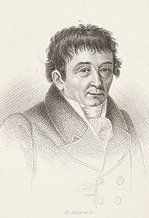
\includegraphics[height=\the\HauteurDesPhotos]{Chladni}&
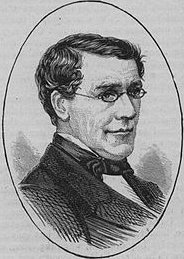
\includegraphics[height=\the\HauteurDesPhotos]{Wheatstone}&
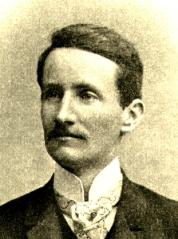
\includegraphics[height=\the\HauteurDesPhotos]{Ritz}&
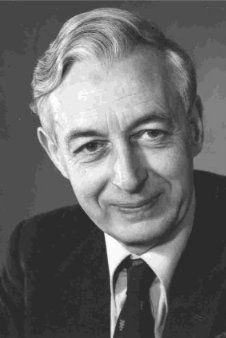
\includegraphics[height=\the\HauteurDesPhotos]{Warburton}&
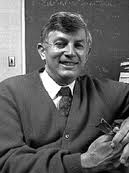
\includegraphics[height=\the\HauteurDesPhotos]{Leissa}\\
Chladni&Wheatstone&Ritz&Warburton&Leissa%
\end{tabular}}
\medskip
\ImageADroite{%
C'est en 1787 à Leipzig que Chladni\index[aut]{Chladni (Ernst Florens Friedrich), 1756-1827, Allemand} met en évidence expérimentalement la formation de lignes nodales sur une plaque libre avec du sable. Wheatstone\index[aut]{Wheatstone (Charles), 1802-1875, Anglais} et Rayleigh,\index[aut]{Rayleigh (John William Strutt, troisième baron -), 1842-1919, Anglais} respectivement en 1833 et 1873, utiliseront des modes de poutre libre pour essayer de comprendre et d'expliquer les figures de Chladni.\\
\indent
En 1909, Ritz,\index[aut]{Ritz (Walther), 1878-1909, Suisse} toujours sur ce problème de la plaque libre, utilisera pour la première fois la méthode qui porte son nom. Les premiers résultats concernant la plaque encastré ne viendront qu'en 1931, et sont dus à Sezawa.\index[aut]{Sezawa (Katsutada), 1895-1944, Japonais}\\
\indent
En 1939, Igushi développe une méthode pour obtenir certains résultats analytiques, mais les premières synthèses complètes sur les méthodes utilisables pour calculer les fréquences naturelles et les déformées modales de plaques ne viendront qu'en 1954 par Warburton,\index[aut]{Warburton (Geoffrey Barratt), 1924-2009, Anglais} et 1969 par Leissa.\index[aut]{Leissa (Arthur W.), 1932-, Américain}}
\end{histoire}

\medskip
La méthodologie est toujours la même et se base sur la \textcolorblue{technique de séparation des variables} qui permet de dire que les variables d'espace et de temps peuvent être séparées. On écrira donc un déplacement transversal~$w(x,y)$ comme produit d'une fonction dépendant de l'espace~$X(x)$ et d'une fonction dépendant du temps~$T(t)$:~$w(x,t)=X(x)T(t)$. Ainsi, il sera «aisé» de résoudre le problème (en ayant pris en compte les conditions aux limites évidemment).

\medskip
Généralement, dans un premier temps, lors du développement de ces modèles de cordes, barres, poutres, membranes et plaques, l'amortissement n'est pas pris en compte. Les solutions obtenues pour les réponses libres ne présentent donc pas de décroissance de l'amplitude des mouvements dans le temps. Il est possible d'intégrer cet amortissement de plusieurs façons:
\begin{description}
  \item[\textcolorblue{Facteur d'amortissement modal:}] il s'agit de la manière la plus simple d'introduire l'amortissement en incluant un terme dissipatif correspondant à un modèle d'amortissement visqueux sur la fonction dépendant du temps uniquement. \textcolorgris{Dans ce cas, la fonction de dépendance temporelle~$T(t)$, qui avait pour équation différentielle $\ddot{T}_n(t)+\omega^2_nT_n(t)=0$, pour les modes~$n\ge1$, devra désormais répondre à l'équation $\ddot{T}_n(t)+2\xi_n\omega_n\dot{T}_n(t)+\omega^2_nT_n(t)=0$, où~$\xi_n$ est le facteur d'amortissement modal};	
  \item[\textcolorblue{Coefficient d'amortissement dans l'équation d'onde:}]
	un terme dissipatif est introduit directement dans l'équation des ondes. Celui-ci peut être proportionnel au milieu externe dans lequel se produit le phénomène \textcolorgris{(par exemple proportionnel à la vitesse de déformation hors plan d'une membrane vibrant dans un fluide, comme l'air)}, ou proportionnel au milieu interne considéré \textcolorgris{(par exemple proportionnel à la vitesse de fluctuation des contraintes dans une poutre: modèle de Kelvin-Voigt)};
  \item[\textcolorblue{Dissipation aux limites:}] l'amortissement peut également être introduit dans la définition des conditions aux limites, par exemple pour prendre en compte le mode de fixation de la structure. \textcolorgris{(Par exemple, dans le cas des ondes longitudinales dans une barre, on introduit un ressort et un amortisseur à chaque bout de la barre).}
\end{description}

Ces remarques, bien que générales, nécessitent d'être correctement prises en compte pour ces modèles simplifiés.


\medskip
\section{Pour aller plus loin: cas des chocs large bande}\label{Sec-choc}

\textcolorgreen{On s'intéresse au cas des chocs, car il constituent un cas plus compliqué que de la «dynamique lente», sans rien enlever en généralité aux méthodes.}

\medskip
\textcolorred{En dynamique transitoire, lorsque le contenu fréquentiel de la sollicitation est large, on montre que les erreurs numériques faites sur chaque longueur d'onde se cumulent, d'où une dégradation de la qualité attendue du résultat plus rapide que prévue.}
De plus, une erreur sur la périodicité des oscillations due à un trop faible nombre de pas de temps et un déphasage des oscillations à cause de cette accumulation des erreurs numériques au cours des pas de temps peuvent être observées.

Dans de tels cas, il est possible de \textcolorblue{se placer dans le domaine fréquentiel}\index{domaine! fréquentiel} (à l'aide de la FFT),\index{transformée de Fourier} ce qui conduit à résoudre un problème de vibrations forcées sur une très large bande de fréquences incluant à la fois les basses et les moyennes fréquences pour l'étude des chocs. La solution temporelle est ensuite reconstruite par transformée de Fourier\index[aut]{Fourier (Jean Baptiste Joseph), 1768-1830, Français}\index{transformée de Fourier} inverse.

Les deux domaines fréquentiels ayant des propriétés différentes, on recourt à des \textcolorblue{outils de résolution différents.}

\medskip
Dans le domaine des \textbf{basses fréquences}, les phénomènes vibratoires générés par l'excitation ont une longueur
d'onde grande face à la structure donc uniquement quelques oscillations sont observables. De plus
la structure présente un comportement modal (modes bien distincts les uns des autres).
La modélisation est maîtrisée: \textcolorblue{éléments finis} sur base modale, complété si besoin de modes
statiques.

\medskip
Pour les \textbf{hautes fréquences}, les longueurs d'ondes sont petites et une centaine d'oscillations est présente sur une dimension de la structure. Il n'est pas approprié de regarder les grandeurs locales, mais plutôt les grandeurs moyennées en espace et en fréquence. On utilise généralement la \textcolorblue{SEA} \index{SEA} qui donne un niveau énergétique vibratoire moyen par sous-structure. Cette méthode ne permet pas d'obtenir une solution prédictive car elle requiert la connaissance \emph{a priori} de facteurs de
couplages mesurés.

\medskip
En \textbf{moyennes fréquences}, plusieurs dizaines d'oscillations apparaissent sur une dimension de la structure, et la déformée est très sensible aux conditions aux limites et aux paramètres matériaux de la structure. Si un comportement modal est encore visible, les modes sont moins bien séparés (par exemple plusieurs modes présents par Hertz, ces modes étant couplés par l'amortissement): la méthode des éléments finis est mal adaptée à cause du raffinement de maillage nécessaire, et le calcul de la base modal est également hors de portée. Les méthodes énergétiques quant à elles sont trop globales et ne permettent pas une description satisfaisante de la solution.

Si la structure est divisible en sous-structures homogènes, on peut utiliser la \textcolorblue{Théorie Variationnelle des Rayons Complexes (TVRC)}\index{Théorie Variationnelle des Rayons Complexes} introduite par Ladevèze en 1996~\cite{bib-Lad96}:\index[aut]{Ladevèze (Pierre), ?- , Français} les conditions de continuité en déplacements et en efforts aux interfaces entre sous-structures n'ont pas besoin d'être vérifiées à priori, mais uniquement au sens faible par une formulation variationnelle.

La TVRC permet l'utilisation d'approximations indépendantes par sous-structure. La solution est supposée bien décrite par la superposition d'un nombre infini de modes locaux, appelés rayons, issus de la vérification des équations d'équilibre dynamique et des relations de comportement par sous-structure. Ces rayons sont à deux échelles: une lente et une rapide. L'échelle rapide est traitée analytiquement (sinon coût numérique élevé), et l'échelle lente numériquement, car elle conduit à un problème à faible nombre d'inconnues.

On profitera de la rapide dispersion des modes moyennes fréquences dans les milieux dispersifs amortis ainsi que de la version large bande de la TVRC développée en 2004 et 2005~\cite{Lit-Chevreuil}\index[aut]{Chevreuil (Mathilde), ?- , Française}

\medskip
\subsection{Approches temporelles}\index{domaine! temporel}

\subsubsection{Discrétisation spatiale}
Une discrétisation par la méthode des éléments finis est mal adaptée aux phénomènes à fort gradient tels que les chocs, car il faut soit un maillage très fin, soit une interpolation par des polynômes de degré élevé, ce qui dans les deux cas augmente considérablement l'effort de calcul.

Étant donné le caractère très localisé des ondes propagatives en dynamique transitoire, la \textcolorblue{méthode des éléments finis adaptatifs} répond au besoin d'enrichir le modèle localement en raffinant le maillage uniquement sur les fronts d'onde de manière contrôlée et automatique.

Ces méthodes recourent à un estimateur d'erreur \emph{a priori}:
\begin{itemize}
	\item estimateur construit sur les résidus d'équilibre pour l'adaptation de
		maillage dans le cadre de la propagation d'ondes;
	\item estimateur utilisant le lissage des contraintes;
	\item estimateur basé sur l'erreur en relation de comportement.
\end{itemize}

\medskip
\subsubsection{Décomposition de domaine en dynamique transitoire}\label{Sec-Schur}

Le domaine est décomposé en sous-domaines plus petits à calculer. On pourra se servir de la parallélisation du problème. \textcolorblue{Le problème est donc condensé sur les quantités d'interface entre sous-domaines, ce qui conduit à un problème de taille réduite.}

La plupart des méthodes utilisées sont des méthodes sans recouvrement; elles peuvent être primales, duales ou mixtes. Le problème d'interface est résolu de façon itérative, ce qui évite la construction explicite du complément de Schur\footnote{En algèbre linéaire et plus précisément en théorie des matrices, le complément de Schur\index{complément de Schur}\index[aut]{Schur (Issai), 1875-1941, Russe} est défini comme suit. Soit:
\begin{equation} \MM{M}=\MM*{\MM{A} & \MM{B} \\ \MM{C} & \MM{D}} \end{equation}
une matrice de dimension~$(p+q)\times(p+q)$, où les blocs~$\MM{A}$, $\MM{B}$, $\MM{C}$, $\MM{D}$ sont des matrices de dimensions respectives~$p\times p$, $p\times q$, $q\times p$ et~$q\times q$, avec~$\MM{D}$ inversible.
Alors, le complément de Schur du bloc~$\MM{D}$ de la matrice~$\MM{M}$ est constitué par la matrice de dimension~$p\times p$ suivante:
\begin{equation} \MM{A}-\MM{B}\MMI{D}\MM{C}\end{equation}

Lorsque~$\MM{B}$ est la transposée de~$\MM{C}$, la matrice~$\MM{M}$ est symétrique définie-positive si et seulement si~$\MM{D}$ et son complément de Schur dans~$\MM{M}$ le sont.}, mais nécessite un taux de convergence élevé pour être efficace.

Dans la méthode duale, les efforts sont privilégiés: la méthode propose à priori des efforts en équilibre aux interface et cherche à écrire la continuité en déplacements. L'inconnue principale, i.e. les inter-efforts entre sous-structures, sont les multiplicateurs de Lagrange aux interfaces.\index[aut]{Lagrange (Joseph Louis, comte de -), 1736-1813, Italien}\index{multiplicateurs de Lagrange}

\medskip
\subsubsection{Discrétisation temporelle}

Les méthodes d'intégration directe sont nombreuses et mieux adaptées que les techniques de bases réduites pour les chocs relativement rapides qui mettent en jeu des fréquences élevées.

Notons qu'il existe des méthodes qui s'affranchissent de la discrétisation temporelle et s'appuient sur une méthode asymptotique numérique pour déterminer la réponse transitoire de la structure; ces méthodes demandent encore à être développées pour les variations temporelles rapides comme les chocs.

Parmi les méthodes d'intégration directes, on utilise classiquement:
\begin{itemize}
	\item les \textcolorblue{schémas de Newmark}\index[aut]{Newmark (Nathan Mortimore), 1910-1981, Américain}\index{schéma! de Newmark} (voir chapitre précédent) pour une intégration d'ordre 2: 		les schémas précis au second ordre des différences centrées et de l'accélération moyenne sont privilégiés pour les faibles erreurs d'amplitude et de périodicité qu'ils engendrent.
		
		Le schéma des différences centrées\index{schéma! des différences finies centrées}
		est explicite et adapté pour les chargements de dynamique rapide et les
		problèmes non linéaires (car la matrice dynamique à inverser est diagonale),
		mais nécessite de vérifier que le signal ne se propage pas de plus d'un élément
		pendant un pas de temps (condition de Courant, ou condition CFL dont nous reparlerons au chapitre suivant).\index[aut]{Courant (Richard), 1888-1972, Américain}
		
		Le schéma de l'accélération moyenne est implicite mais inconditionnellement
		stable, bien adapté pour les chargement peu rapides.
	\item la \textcolorblue{méthode de Galerkine discontinue}:\index[aut]{Galerkine (Boris), 1871-1945, Russe}\index{méthode de Galerkine! discontinue}
		Elle autorise les variables du problème déplacement et vitesse à être
		discontinues en temps.
		À l'ordre zéro (champs constants sur chaque intervalle de temps), elle permet
		de s'affranchir des oscillations numériques occasionnées lors du traitement
		d'un front d'onde.
		Toutefois, ce schéma dissipe énormément et demande une discrétisation
		très fine pour bien représenter les irrégularités.
	\item la \textcolorblue{TXFEM (Time eXtended FEM)}:\index{TXFEM}
		Elle utilise une base de fonctions de forme en temps enrichie formant une partition de l'unité. Le schéma est équivalent à certaines méthodes de Galerkine discontinues, le nombre de pas de temps inférieur à Newmark, et les oscillations numériques atténuées.
		Elle est bien adaptée pour le traitement des discontinuités en temps et
		notamment les chocs. Voir le paragraphe~\ref{Sec-XFEM} pour une courte description.
\end{itemize}

\medskip
\subsection{Approches fréquentielles}\index{domaine! fréquentiel}

Afin de s'affranchir de l'intégration temporelle et des soucis numériques associés, il est possible de réécrire le problème temporelle en un problème fréquentiel (grâce à la FFT).\index{transformée de Fourier}

\textcolorblue{L'approche fréquentielle est également plus adaptée dans les situations pour lesquelles des paramètres physiques dépendent de la fréquence.}\index{domaine! fréquentiel}

\medskip
En appliquant la transformée de Fourier\index[aut]{Fourier (Jean Baptiste Joseph), 1768-1830, Français}\index{transformée de Fourier} à toutes les quantités dépendant du temps, on obtient des quantités qui dépendent de la fréquence. Ce faisant, le problème à résoudre devient un problème de vibration forcée sur une bande de fréquence. Il faut alors calculer des fonctions de réponse en fréquence (FRF)\index{FRF} sur une large plage de fréquences.

\medskip
\subsubsection{Cas des basses fréquences}

Compte tenu de la grande taille des longueurs d'ondes et du fait que l'on a peu de modes, bien séparés, les méthodes utilisées sont basées sur les \textcolorblue{éléments finis}.

En réécrivant le problème dynamique dans le cas d'une sollicitation harmonique de pulsation $\omega$, il vient (comme nous venons de le présenter avant):
\begin{equation}
\left(-\omega^2\MM{M}+i\omega \MM{C}+\MM{K}\right)\VV{q} = \VV{F}
\end{equation}

En utilisant \textcolorblue{l'hypothèse de Basile}\footnote{%
Si le seul amortissement entrant en jeu est un amortissement structurel (dissipation
interne du matériau pour une structure homogène), il est alors licite de faire
l'hypothèse d'un amortissement proportionnel, encore appelé hypothèse de
Basile. Dans ce cas~$\MM{C}$ s'exprime comme combinaison linéaire de~$\MM{M}$ et~$\MM{K}$,
et sa projection sur les modes propres est diagonale.
} sur l'amortissement, il est possible de calculer les premiers modes propres\index{mode propre} associés aux plus petites fréquences propre\index{fréquence propre} du système. La solution approchée est alors projetée sur les sous-espaces propres\index{espace!propre} associés. On résout alors un système diagonale de petite taille.

\medskip
\subsubsection{Cas des moyennes fréquences}

En moyennes fréquences, l'approche précédente (par éléments finis) nécessiterait d'utiliser une grande quantité de polynômes à cause du caractère très oscillant, ou à augmenter le degré d'interpolation. De plus, il faut prendre en compte plus de modes, qui sont de moins en moins bien séparés.

\medskip
Notons que l'on peut minimiser l'influence du raffinage du maillage en localisant celui-ci uniquement où la dynamique locale le demande. Pour cela, des estimateurs d'erreur \emph{a posteriori} ont été développés pour les structures, mais également pour l'acoustique.

La dispersion numérique est moindre avec les éléments finis stabilisés: tels que les \textcolorblue{Galerkin Least Squares} et \textcolorblue{Galerkin Gradient Least Squares}\index{méthode de Galerkine! Least Squares}\index{méthode de Galerkine! Gradient Least Squares}... qui n'intervienne pas sur la forme variationnelle mais sur les matrices issues de celle-ci.

\medskip
On peut également essayer de diminuer la taille de la base modale à prendre en compte en ne retenant que les modes propres qui maximisent l'opérateur d'excitabilité; mais pour cela il faut d'abord calculer la base complète...

On peut également utiliser un autre espace de projection que les modes propres classiques: par exemple les premiers modes d'un opérateur d'énergie relatif à une bande de fréquence (Soize 98 \cite{bib-Soize98}).\index[aut]{Soize (Christian), 1948- , Français} Cette approche peut être couplée à la \textcolorblue{théorie des structures floues}\index{théorie des structures floues} (Soize 86 \cite{bib-Soize86}) pour prendre en compte la complexité de la structure de manière probabiliste.

\medskip
On peut également sous-structurer le domaine. Dans la \textcolorblue{Component Modal Synthesis},\index{Component Modal Synthesis} les modes propres\index{mode propre} de chaque sous-structures servent de base pour la solution de la structure entière.

\bigskip
Une «deuxième» approche consiste à utiliser des \textcolorblue{éléments enrichis}\index{élément fini!enrichi} (voir encore une fois le chapitre~\ref{Ch-XFEM}). Ces éléments sont développés pour pouvoir prendre en compte le caractère oscillant de la solution en enrichissant les fonctions de base utilisées afin de pouvoir mieux reproduire la solution.

\medskip
Les \textcolorblue{éléments finis hiérarchiques,\index{élément fini!hiérarchique} issus des méthodes~$p$}\index{méthode~$p$} (voir le paragraphe~\ref{Sec-rhp}: \textcolorgreen{l'augmentation du degré polynomial des fonctions de forme peut se voir comme une substitution à un raffinement de maillage, mais les estimateurs d'erreur des méthodes~$p$ sont meilleurs que ceux des méthodes~$h$}),\index{méthode~$h$}\index{méthode~$p$} permettent une réutilisation à l'ordre~$p+1$ des matrices de masse et de raideur élémentaires issues de l'ordre~$p$.

Les \textcolorblue{éléments finis multi-échelles} (voir paragraphe~\ref{Sec-ssstruc}) où la solution est recherchée comme somme d'une composante calculable à l'échelle grossière en espace et d'une composante non calculable associée à l'échelle fine.

La \textcolorblue{Méthode de partition de l'unité (PUM)}\index{partition de l'unité} (voir paragraphe~\ref{Sec-partition}) utilise un recouvrement du domaine initial en un ensemble de maillages, chacun étant enrichi et vérifiant la partition de l'unité. La méthode des éléments finis associée à la méthode de partition de l'unité donne naissance à deux grandes familles d'approches: la G-FEM (Generalized FEM)\index{G-FEM} et la X-FEM (eXtended FEM),\index{X-FEM}\index{méthode des éléments finis étendue} voir paragraphe~\ref{Sec-XFEM}. Si les fonctions d'enrichissement ne sont pas activées, on se retrouve avec la méthode des éléments finis classique.

la \textcolorblue{Méthode d'enrichissement discontinu}\index{méthode d'enrichissement discontinu} (Discontinuous Enrichment Method) est une méthode de Galerkine éléments finis discontinue avec multiplicateurs de Lagrange\index{méthode de Galerkine!discontinue!avec multiplicateurs de Lagrange} dédiée aux application de forts gradients ou oscillations rapides.

\bigskip
La \textcolorblue{méthode des éléments frontières}\index{élément fini!frontière} ou BEM (voir paragraphe~\ref{Sec-BEM}) est encore une «troisième» approche. Seuls les bords sont maillés afin de réduire le nombre de degrés de liberté. La formulation intégrale de la frontière établit un lien entre les champs intérieurs et les quantités sur les bords. La matrice obtenue est petite, mais pleine et non symétrique.

\bigskip
Les \textcolorblue{méthodes sans maillage}\index{méthode sans maillage} (voir paragraphe~\ref{Sec-meshless}): Dans la EFGM (Element Free Galerkin Method ou méthode de Galerkine sans maillage),\index{méthode de Galerkine!sans maillage} on n'a plus qu'un nuage de points sans connectivité entre eux. On utilise des fonctions de formes construites selon la méthode des moindres carrés mobiles et formant une partition de l'unité,\index{partition de l'unité} qui peuvent être polynomiales ou sinusoïdales. Néanmoins, comme elle est basée sur une discrétisation nodale, elle nécessite également un grand nombre de nœuds aux fréquences plus élevées.

\bigskip
Les \textcolorblue{méthodes des éléments discontinus}:\index{méthode des éléments discontinus} Pour des géométries simples (utilisation en construction navale), on utilise des solutions analytiques ou semi-analytiques sur des sous-domaines simples (poutres, plaques rectangulaires...) pour construire la structure complète. Lorsque cette méthode est applicable \textcolorblue{elle donne de bon résultats aussi bien en basses fréquences, en moyennes fréquences et en hautes fréquences}.

\bigskip
Les \textcolorblue{méthodes de Trefftz}:\index{méthode de Trefftz}\index[aut]{Trefftz (Erich Immanuel), 1888-1937, Allemand} Elles utilisent des fonctions de base définies sur tout le domaine de la sous-structure considérée et vérifiant exactement l'équation dynamique et la loi de comportement: la solution est représentée par la superposition de ces fonctions; mais il faut encore vérifier les conditions aux limites et de transmission. Les matrices sont de petite taille mais très mal conditionnées.

Les T-éléments lient la démarche Trefftz\index[aut]{Trefftz (Erich Immanuel), 1888-1937, Allemand} et la méthode des éléments finis: Trefftz au sein de chaque élément..

Pour les problèmes de \textcolorblue{vibroacoustique}, la \textcolorblue{WBT (Wave Based Technique)}\index{WBT} a été développée: la structure n'est pas discrétisée comme pour les T-éléments mais est décomposée en éléments de grande taille par rapport à la dimension de la structure. les fonctions de base particulières utilisées améliorent le conditionnement des matrices, ce qui conduit à des matrices de petite taille pleines et non symétriques. L'intégration sur les bords coûte cher en moyennes fréquences et le conditionnement de la matrice en hautes fréquences se dégrade du fait de la discrétisation des amplitudes (seules certaines directions de propagation sont prises en compte).

\medskip
\subsubsection{Cas de hautes fréquences}

Comme dit précédemment, on ne représente pas la solution localement mais on ne s'intéresse qu'à des grandeurs moyennées.

\bigskip
La \textcolorblue{SEA\index{SEA} (Statistical Energy Analysis) est la méthode de référence pour les hautes fréquences}. La structure est découpée en sous-structures. Ensuite des regroupements de modes sont construits tels que statistiquement le niveau de chacun des groupes de modes soit semblable: la méthode repose donc sur l'hypothèse d'une forte densité modale dans la bande de fréquence étudiée. Chaque groupe de mode est associé à un degré de liberté: le problème à résoudre issu de l'équilibre énergétique est par conséquent à faible nombre de degrés de liberté. Cet équilibre se traduit par un bilan de puissance dans lequel la puissance injectée à une sous-structure par des forces extérieures, aléatoires et stationnaires sur de larges bandes de fréquences, est égale à la somme de la puissance dissipée dans cette sous-structure par amortissement et la puissance transmise à l'ensemble des sous-structures voisines avec lesquelles elle est connectée, appelée puissance de couplage. \textcolorred{L'hypothèse forte de la SEA\index{SEA} concerne cette puissance de couplage entre deux sous-structures qui est supposée proportionnelle à la différence de leurs énergies par mode,\index{mode propre} le facteur de proportionnalité étant le coefficient de couplage.}

La SEA\index{SEA} est parfaitement adaptée aux hautes fréquences, mais trop globale et trop imprécise pour décrire finement le comportement en moyennes fréquences.

De plus les coefficients de couplages ne sont connus explicitement \emph{a priori} que pour des géométries très particulières et nécessitent donc en général de recourir à des expériences, ce qui fait de la SEA\index{SEA} une méthode non prédictive.

Des stratégies de calcul de ces coefficients de couplage existent, mais pour certains régimes d'excitation la notion même de coefficient de couplage n'est plus réaliste.

\bigskip
La \textcolorblue{méthode de diffusion d'énergie}:\index{méthode de diffusion d'énergie} Elle apporte un effet local à la SEA\index{SEA} en décrivant de manière continue les variables énergétiques. Elle a été appliquée à des cas simples et l'analogie avec la thermique n'est pas démontrée pour des sollicitations et des géométries quelconques. 

\bigskip
L'\textcolorblue{analyse ondulatoire de l'énergie}:\index{analyse ondulatoire de l'énergie} Elle généralise la SEA\index{SEA} en ce qu'elle considère le champ d'ondes non plus diffus mais directionnel en introduisant un champ d'ondes aléatoires propagatives dans les sous-structures et des coefficients de couplages qui varient selon les angles
d'incidence aux interfaces.

\bigskip
Les \textcolorblue{Méthodes Énergétiques Simplifiées} ou MES:\index{méthodes Énergétiques Simplifiées} Elles se proposent de pallier les insuffisances de la méthode de diffusion de l'énergie en donnant une représentation locale des phénomènes. Le bilan de puissance est écrit aussi bien à l'intérieur des sous-structures que de leurs couplages. La connaissance des coefficients de couplages \emph{a priori} demeure un problème.

\bigskip
D'autres méthodes existent encore: développements asymptotiques, méthode de l'enveloppe, méthode des chemins structuraux.

La \textcolorblue{méthode des rayons}:\index{méthode des rayons} consiste à suivre les rayons vibratoires le long de leur parcours par l'étude de leur propagation, réflexion et transmission entre sous-structures par les lois de Snell-Descartes\index[aut]{Snell (Snell van Royen (Willebrord), dit Villebrordus Snellius ), 1581-1626, Néerlandais}\index[aut]{Descartes (René), 1596-1650, Français}\footnote{Selon Huygens,\index[aut]{{Huygens [ou Huyghens] (Christian), 1629-1695, Néerlandais}} Snell découvrit le premier les lois de la réfraction en 1621. Il semble par ailleurs qu'on lui doive également, avant Neper,\index[aut]{Neper [ou Napier] (John, Baron de Merchiston), 1550-1617, Écossais} l'écriture actuelle des nombres décimaux, en France tout au moins: $e,dcm...$ distinguant, séparées par une virgule, les parties entière~$e$ et décimale ($d$ = dixièmes, $c$ = centièmes, $m$ = millièmes,... ).} de l'optique géométrique jusqu'à l'amortissement des ondes. La RTM permet de connaître la direction privilégiée de transfert et de répartition spatiale de l'énergie, mais à un coût numérique très élevé. De plus, les coefficients de transmissions ne sont pas connus à priori...

\medskip
\subsection{Remarques}

Dans l'approche fréquentielle, il faut déterminer les fréquences déterminant la jonction BF/MF et MF/HF.

La fréquence BF/MF agit sur le coût de calcul: elle doit être la plus grande possible, mais telle qu'à partir de cette fréquence, les modes de la structure deviennent locaux, tout en conservant la séparation des modes (en pratique entre 300 et 600 Hz).

Le choix de la fréquence MF/HF joue sur la qualité de la vitesse calculée et donc sur l'énergie cinétique qui sert pour restaurer la réponse temporelle. Cette fréquence doit être au moins égale à~$1/T$ où $T$ est la durée du choc d'entrée (si~$T=1$~ms, alors MF/HF = 2000~Hz mini).

la méthode des éléments finis utilisée en basses fréquences doit utiliser les~$n$ premiers modes pour la base réduite avec~$n$ tel que la fréquence de ce mode soit de~$2\times$ la fréquence BF/MF. On utilisera également la règle classique d'\textcolorblue{au moins 10 éléments linéaires par longueur d'onde pour le maillage}.

La FFT\index{transformée de Fourier} requiert par ailleurs que le chargement soit périodique. Le temps correspondant à cette période, $T_0$, doit être choisi judicieusement. Dans le cas d'un choc, on a donc~$T_0 > T$, mais il faut également le choisir tel que la réponse transitoire de la structure s'éteigne avant la fin de cet intervalle de temps. De plus, ce temps influe sur l'échantillonnage fréquentiel du calcul de la FRF. Les pulsations pour lesquelles la FRF est calculée doivent être telles que~$\omega_n=2\pi n f_0$ avec~$f_0=1/T_0$. Il faut également que le nombre de pas de fréquences~$N$ soit une puissance de 2 pour utiliser la FFT\index{transformée de Fourier} et son efficacité, et~$N$ soit être tel que~$N/T_0 \ge 2 f_{\max}$ avec~$f_{\max}$ la fréquence maximale contenue dans le signal.

\medskip
Le choix judicieux de~$T_0$ influe directement sur la reconstruction temporelle de la réponse. Pour les structures peu amorties ou pour des chargements longs, $T_0$ est grand, et donc la FFT\index{transformée de Fourier} coûteuse. Dans ces cas, des méthodes ont été développées: les fonctions de Green;\index[aut]{Green (George), 1793-1841, Anglais} la Implicit Fourier Transform; et l'amortissement artificiel.

